\documentclass[letterpaper,11pt]{article}
\usepackage{listings}
\usepackage[pdftex]{graphicx} 
\usepackage[utf8]{inputenc}
%\usepackage[english]{babel}
\usepackage{alltt}
\usepackage{color}
\usepackage{url}
\usepackage[T1]{fontenc}
\usepackage{float}
\usepackage{hyperref}
\usepackage{longtable}
\usepackage{caption}
\usepackage{spverbatim}
\usepackage[table,xcdraw]{xcolor}
\usepackage{multirow}

\definecolor{dkgreen}{rgb}{0,0.6,0}
\definecolor{gray}{rgb}{0.5,0.5,0.5}
\definecolor{mauve}{rgb}{0.58,0,0.82}
\definecolor{codegreen}{rgb}{0,0.6,0}
\definecolor{codegray}{rgb}{0.5,0.5,0.5}
\definecolor{codepurple}{rgb}{0.58,0,0.82}
\definecolor{backcolour}{rgb}{0.95,0.95,0.92}

\addtolength{\textwidth}{4cm}
\addtolength{\hoffset}{-2cm}
\addtolength{\textheight}{4cm}
\addtolength{\voffset}{-2cm}

\lstdefinestyle{mystyle}{
    backgroundcolor=\color{backcolour},   
    commentstyle=\color{codegreen},
    keywordstyle=\color{magenta},
    numberstyle=\tiny\color{codegray},
    stringstyle=\color{codepurple},
    basicstyle=\footnotesize,
    breakatwhitespace=false,         
    breaklines=true,                 
    captionpos=b,                    
    keepspaces=true,                 
    numbers=left,                    
    numbersep=5pt,                  
    showspaces=false,                
    showstringspaces=false,
    showtabs=false,                  
    tabsize=2
}

\lstset{style=mystyle}

\lstset{
	basicstyle=\footnotesize,
	breaklines=true,
}

\title{Bibliography management: BibTeX}
\author{Share\LaTeX}

\begin{document}

\begin{titlepage}

\begin{center}

\Huge{Assignment 3}

\Large{CS834-F16:  Introduction to Information Retrieval}

\Large{Fall 2016}


\Large{Erika Siregar}

\vfill

% Bottom of the page
\Large{CS Department - Old Dominion University  \\ \today}


\end{center}

\end{titlepage}


\section*{Question 6.1}
\begin{spverbatim}
Using the Wikipedia collection provided at the book website, create a sample of stem clusters by the following process:
1. Index the collection without stemming.
2. Identify the first 1,000 words (in alphabetical order) in the index.
3. Create stem classes by stemming these 1,000 words and recording which words become the same stem.
4. Compute association measures (Dice’s coefficient) between all pairs of stems in each stem class. Compute co-occurrence at the document level.
5. Create stem clusters by thresholding the association measure. All terms that are still connected to each other form the clusters.

Compare the stem clusters to the stem classes in terms of size and the quality (in your opinion) of the groupings.
\end{spverbatim}

\subsection*{Answer}
For indexing the collection, I modified the code that I used in assignment 2, sort the index alphabetically, and take the first 1000 words. The code for this is written in the file `1\_2\_index.py'. For creating the stem classes, I use Krovetz Stemmer because it produces a better stemming results than Porter Stemmer. Listing \ref{lst:krovetz} shows the code to create the stem classes that utilize python library for Krovetz Stemmer \cite{krovetz-python}.

\begin{lstlisting}[language=python, caption={Creating Stem Classes with Krovetz Stemmer}, label={lst:krovetz}]
#!/usr/bin/python
import json
from krovetzstemmer import Stemmer as KrovetzStemmer
import unicodecsv as csv
from prettyprint import prettyprint


# Instantiate krovetz stemmer
krovetz = KrovetzStemmer()


# Read result of 1_index
with open('1_2_index.txt', 'rb') as f:
    str_word_files_index = f.read()
    word_files_index =  json.loads(str_word_files_index)

    stem_word_index = {}
    for word, files in word_files_index.items():
        # Stem word using krovetz
        stemmed_word = krovetz.stem(word)

        # Group by stemmed word
        stem_word_index.setdefault(stemmed_word, [])
        stem_word_index[stemmed_word].append(word)


    filename = '3_stemmed_words.csv'
    with open(filename, 'wb') as f:
        print('Writing to file {}'.format(filename))

        writer = csv.writer(f)
        for stemmed_word, words in stem_word_index.items():
            writer.writerow((stemmed_word, ', '.join(words)))

        print('Done!')

\end{lstlisting}

Table \ref{tab:stem-class} shows the snippet of the stem classes created. The complete list of the stem classes is available in `3\_stemmed\_words.csv' which is uploaded on github. 

\begin{table}[H]
\centering
\begin{tabular}{|l|l|}
\hline
\multicolumn{1}{|c|}{\textbf{stem class}} & \multicolumn{1}{c|}{\textbf{terms}}      \\ \hline
academician                          & academicians, academician                \\ \hline
adamant                              & adamantly, adamant                       \\ \hline
abundance                            & abundance                                \\ \hline
account                              & account, accounted, accounts, accounting \\ \hline
abdelkader                           & abdelkader                               \\ \hline
achter                               & achter                                   \\ \hline
abednego                             & abednego                                 \\ \hline
abortion                             & abortion, abortions                      \\ \hline
aboot                                & aboot                                    \\ \hline
abrahamsson                          & abrahamsson                              \\ \hline
abdeali                              & abdeali                                  \\ \hline
abandon                              & abandonment, abandon, abandoning         \\ \hline
\end{tabular}
\caption{A snippet of the stem classes}
\label{tab:stem-class}
\end{table}
 
Next step is to create the stem clusters using Dice's Coefficient \cite{dice} as the term association measure. Dice's Coefficient works based on this formula: \[ 2.\frac{n_{ab}}{n_{a} + n_{b}} \]      
Using this formula, compute the Dice's Coefficient for each pair of terms in every stem classes. With a threshold = 0.01, create a graph in which every pair of terms that has Dice's Coefficient greater than 0.01 will be connected with an edge. Figure \ref{fig:4_graph_activate} shows the graph for the stem class `activate' that can be grouped into two clusters: `\textit{activate, activating, activator}' and `\textit{activates, activation}'. The graph for other stem classes are available on github in a folder named \textit{`graph'}. From this graph, we only need to extract the connected components to form the clusters. \newline
Listing \ref{lst:cluster} shows the code used to compute the Dice's Coefficient, create the graphs, and extract the connected components of the graphs. 

\begin{lstlisting}[language=python, caption={Creating Cluster using Dice's Coefficient}, label={lst:cluster}]

#!/usr/bin/python
import json
import nltk as nltk
from tabulate import tabulate
import unicodecsv as csv
from prettyprint import prettyprint
import networkx as nx
import matplotlib.pyplot as plt

dice_coef_threshold = 0.01
stem_clusters = []

# Read result of 1_2_index.txt
with open('1_2_index.txt', 'rb') as f1:
    word_files_index = json.loads(f1.read())

    # Read result of 3_stemmed_words.csv
    with open('3_stemmed_words.csv', 'rb') as f3:
        for stemmed_word, words in csv.reader(f3):
            words = words.split(', ')

            # create bigrams from words
            bigrams = list(nltk.bigrams(words))
            for word_a, word_b in bigrams:
                # Lookup filename in word_files_index
                files_a = word_files_index[word_a]
                files_b = word_files_index[word_b]
                files_a_sliced_b = list(set(files_b) & set(files_a))

                dice_coef = float(2 * len(files_a_sliced_b)) / (len(files_a) + len(files_b))

                if(dice_coef > dice_coef_threshold):
                    stem_clusters.append((stemmed_word, word_a, word_b, dice_coef))


stem_clusters = sorted(stem_clusters, key=lambda x: x[3], reverse=True)
# print tabulate(stem_clusters, headers=['stemmed_word', 'word_a', 'word_b', 'dice_coef'])

filename = '4_dice_coeficient.csv'
with open(filename, 'wb') as f:
    print('Writing to file {}'.format(filename))

    writer = csv.writer(f)
    for stemmed_word, word_a, word_b, dice_coef in stem_clusters:
        writer.writerow((stemmed_word, word_a, word_b, dice_coef))


# Create graph
stemmed_word_data = {}
for stemmed_word, word_a, word_b, dice_coef in stem_clusters:
    stemmed_word_data.setdefault(stemmed_word, [])
    stemmed_word_data[stemmed_word].append((word_a, word_b, dice_coef))

stemmed_word_clusters = {}
for stemmed_word, data in stemmed_word_data.items():
    G=nx.MultiGraph()

    labels = {}
    for word_a, word_b, dice_coef in data:
        G.add_edge(word_a, word_b, weight=dice_coef, label=dice_coef)
        labels[(word_a, word_b)] = dice_coef

    # export connected components into list
    stemmed_word_clusters[stemmed_word] = list(nx.connected_components(G))

    nx.draw(G, with_labels=True)
    nx.draw_networkx_edge_labels(G, pos=nx.spring_layout(G), edge_labels=labels)

    filename = '4_graph_{}.png'.format(stemmed_word)
    print('Saving graph {}'.format(filename))
    plt.savefig(filename, format='PNG')
    plt.clf()

print('Draw graphics done!')

print('Print stem clusters...')

for stemmed_word, connected_nodes in stemmed_word_clusters.items():
    for connected_node in connected_nodes:
        print(u'{}\t: {}'.format(stemmed_word, ', '.join(connected_node)))

print('Print stem clusters done')


\end{lstlisting}

\begin{figure}[H]
	\fbox{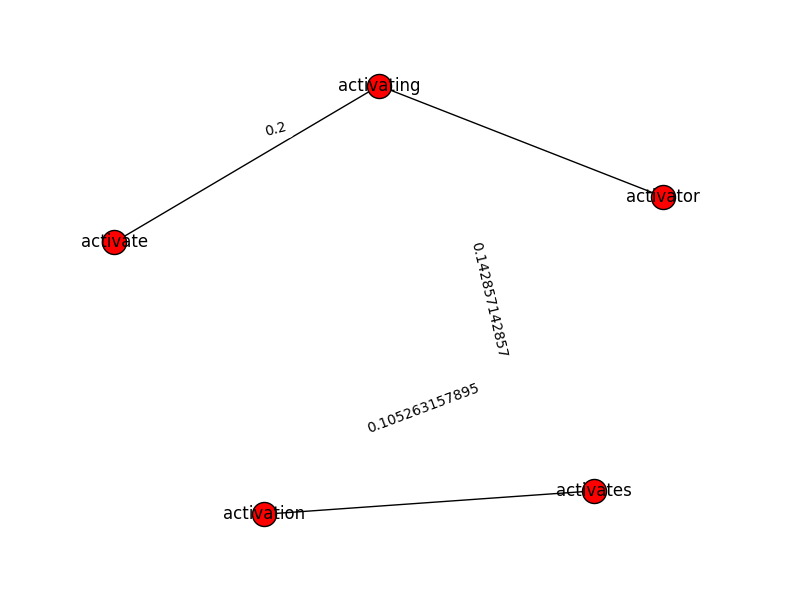
\includegraphics[scale=0.7]{4_graph_activate}}
	\centering
	\caption{Graph of the connected component for the stem class `activate'}
	\label{fig:4_graph_activate}
\end{figure}

Table \ref{tab:dice} shows the Dice's Coefficient for some pair of terms in the Wikipedia collection. The complete list of the term pairs with their Dice's Coefficient value is available on Github in a file named `4\_dice\_coeficient.csv'. 

\begin{table}[H]
\centering
\begin{tabular}{|l|l|l|l|l|}
\hline
No & \multicolumn{1}{c|}{\textbf{Class}} & \multicolumn{1}{c|}{\textbf{Term 1}} & \multicolumn{1}{c|}{\textbf{Term 2}} & \multicolumn{1}{c|}{\textbf{Dice's Coefficient}} \\ \hline
1  & abomination                         & abominationes                        & abomination                          & 0.6666666667                                     \\ \hline
2  & abut                                & abuts                                & abutting                             & 0.6666666667                                     \\ \hline
3  & abjad                               & abjads                               & abjad                                & 0.6666666667                                     \\ \hline
4  & academician                         & academicians                         & academician                          & 0.5714285714                                     \\ \hline
5  & aberration                          & aberrations                          & aberration                           & 0.5                                              \\ \hline
6  & adapter                             & adapters                             & adapter                              & 0.5                                              \\ \hline
7  & actor                               & actors                               & actor                                & 0.4984025559                                     \\ \hline
8  & abridge                             & abridged                             & abridges                             & 0.4                                              \\ \hline
9  & absolve                             & absolve                              & absolved                             & 0.4                                              \\ \hline
10 & acoustic                            & acoustically                         & acoustical                           & 0.4                                              \\ \hline
\end{tabular}
\caption{Dice's Coefficient for some pair of terms in small Wikipedia collection}
\label{tab:dice}
\end{table}

Listing \ref{lst:cluster} shows the clusters resulted for the small Wikipedia Collection. 

\begin{lstlisting}[caption={Cluster for the small wikipedia collection}, label={lst:cluster}]
accessible	: accessible, accessibility	
activate	: activator, activate, activating
activate	: activation, activates
accelerator	: accelerators, accelerator
abridge	: abridges, abridged
accurate	: accurate, accurately
address	: addressing, addresses, addressed, address
abomination	: abomination, abominationes
accept	: accepting, accepted, accept
abbreviation	: abbreviation, abbreviations
acclaim	: acclaim, acclaimed
adaptation	: adaptations, adaptation
abrogate	: abrogation, abrogated
accrete	: accreting, accrete, accreted
acid	: acidic, acids, acid
accommodate	: accommodate, accommodated
absolute	: absoluter, absolute
acceleration	: acceleration, accelerations
additional	: additional, additionally
acknowledge	: acknowledges, acknowledged
addition	: addition, additions
accent	: accent, accented
actor	: actors, actor
access	: access, accessed, accessing, accessor
acyltransferase	: acyltransferase, acyltransferases
add	: adding, add, added, adds
activist	: activist, activists
adapt	: adaption, adapt
adapt	: adaptive, adapted
acre	: acres, acre
achieve	: achieves, achieve
achieve	: achieving, achieved
abstraction	: abstraction, abstractions
accompany	: accompany, accompanying
activity	: activities, activity
accidental	: accidentally, accidental
aberration	: aberrations, aberration
acronym	: acronym, acronyms
academy	: academy, academies
acquire	: acquire, acquiring
academician	: academician, academicians
abut	: abutting, abuts
abuse	: abused, abuse
accompaniment	: accompaniment, accompaniments
actress	: actresses, actress
accuse	: accusing, accuses
acute	: acute, acutely
accumulate	: accumulate, accumulated
abugida	: abugidas, abugida
abduct	: abducted, abductors
achievement	: achievements, achievement
accredit	: accrediting, accredited, accreditation
accusation	: accusation, accusations
account	: accounting, accounted, accounts
accident	: accident, accidents
actual	: actual, actualized
adapter	: adapter, adapters
accomplishment	: accomplishment, accomplishments
absolve	: absolved, absolve
abjad	: abjads, abjad
academic	: academic, academically
abrupt	: abrupt, abruptly
abolition	: abolitionism, abolition
act	: acted, act
action	: action, actions
acoustic	: acoustical, acoustic, acoustically
abbey	: abbeys, abbey
acquisition	: acquisitions, acquisition
abbot	: abbots, abbot

\end{lstlisting}

\noindent\makebox[\linewidth]{\rule{\textwidth}{0.4pt}}

\section*{Question 6.2}
\begin{spverbatim}
Create a simple spelling corrector based on the noisy channel model. Use a single-word language model, and an error model where all errors with the same edit distance have the same probability. Only consider edit distances of 1 or 2. Implement your own edit distance calculator (example code can easily be found on the Web).
\end{spverbatim}

\subsection*{Answer:}
Spelling corrector based on the noisy channel model works using this approach \cite{spelling}:
\begin{enumerate}
\item Let's say \textit{x} is a mispelled word and \( w = w_{1}, w_{2}, w_{3}, ..., w_{n} \) is an array of possible corrected words. 
\item Our task is to compute the conditional probability and take a word \( w_i \) that has the maximum value for \( P\left(x|w_{i}\right).P\left(w_i\right) \).
\end{enumerate}

It looks complicated. But, fortunately, Peter Norvig \cite{norvig} has provided a nice python code for spelling corrector, which is worked based on the noisy channel model. To compute the probability, Norvig uses word frequencies taken from a predefined dataset `big.txt'. For this assignment, I modified Norvig's code as can be seen in listing \ref{lst:spelling}.

\begin{lstlisting}[language=python, caption={Spelling corrector}, label={lst:spelling}]

#!/usr/bin/python

import re
from collections import Counter

import sys


class Spell:
    def __init__(self, train_file):
        self.document = open(train_file).read()
        self.to_words()
        self.count_words()

    def to_words(self):
        self.words = re.findall(r'\w+', self.document.lower())

    def count_words(self):
        self.word_count = Counter(self.words)

    def probability(self, word):
        "Probability of `word`."
        word = word.lower()
        N = sum(self.word_count.values())
        return self.word_count[word] / N

    def edits1(self, word):
        "All edits that are one edit away from `word`."
        word = word.lower()
        letters = 'abcdefghijklmnopqrstuvwxyz'
        splits = [(word[:i], word[i:]) for i in range(len(word) + 1)]
        deletes = [L + R[1:] for L, R in splits if R]
        transposes = [L + R[1] + R[0] + R[2:] for L, R in splits if len(R) > 1]
        replaces = [L + c + R[1:] for L, R in splits if R for c in letters]
        inserts = [L + c + R for L, R in splits for c in letters]
        return set(deletes + transposes + replaces + inserts)

    def edits2(self, word):
        "All edits that are two edits away from `word`."
        word = word.lower()
        return (e2 for e1 in self.edits1(word) for e2 in self.edits1(e1))

    def known(self, words):
        "The subset of `words` that appear in the dictionary of WORDS."
        return set(w for w in words if w in self.word_count)

    def candidates(self, word):
        "Generate possible spelling corrections for word."
        word = word.lower()
        return (self.known([word]) or self.known(self.edits1(word)) or self.known(self.edits2(word)) or [word])

    def correction(self, word):
        "Most probable spelling correction for word."
        word = word.lower()
        candidates = self.candidates(word)
        return max(candidates, key=self.probability)


if __name__ == '__main__':
    spell = Spell('big.txt')

    if len(sys.argv) != 2:
        print('python spell.py <word>')
        exit()

    word = sys.argv[1]
    spelled_word = spell.correction(word)

    print('{} --> {}'.format(word, spelled_word))

\end{lstlisting}

Figure \ref{fig:spelling_corrector} shows the example of spelling correction using some words taken from the textbook \cite{Croft:2009:SEI:1516224} and some words taken from Norvig's website \cite{norvig}. 

\begin{figure}[H]
	\fbox{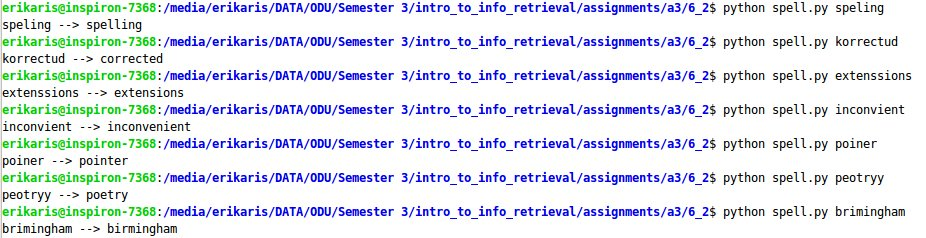
\includegraphics[scale=0.56]{spelling_corrector}}
	\centering
	\caption{Spelling corrector using noisy channel model with edit distance of 1 and 2}
	\label{fig:spelling_corrector}
\end{figure}

\noindent\makebox[\linewidth]{\rule{\textwidth}{0.4pt}}

\section*{Question 6.5}
\begin{spverbatim}
Describe the snippet generation algorithm in Galago. Would this algorithm work well for pages with little text content? Describe in detail how you would modify the algorithm to improve it.
\end{spverbatim}

\subsection*{Answer}
For this question, I downloaded the source code for Galago version 3.10 \cite{galago_3.10} from \url{https://sourceforge.net/p/lemur/galago/ci/release-3.10/tree/}. It is a part of The Lemur Project \cite{lemur}. The code for the snippet generator can be found in a file named \textit{`SnippetGenerator.java'} under the directory `galago-3.10/core/src/main/java/org/lemurproject/galago/core/index/corpus'. This is how the code works:
\begin{enumerate}
\item Given `documentText' and a set of `queryTerms', tokenize the `documentText' into terms and its position. Listing \ref{lst:step1} shows the code for this step. 

\begin{lstlisting}[language=Java, caption={}, label={lst:step1}]

 public String getSnippet(String documentText, Set<String> queryTerms) throws IOException {
    ArrayList<IntSpan> positions = new ArrayList<IntSpan>();
    Document document = parseAsDocument(documentText, positions);
    return generateSnippet(document, positions, queryTerms);
  }

\end{lstlisting}

\item Stem each term using a defined stemmer. By default, Galago uses Krovetz stemmer. 

\begin{lstlisting}[language=Java, caption={}, label={lst:step2}]

  private Document parseAsDocument(String text, ArrayList<IntSpan> positions) throws IOException {
     Document document = new Document();
     document.text = text;
 
     // Tokenize the document
     TagTokenizer tokenizer = new TagTokenizer();
     tokenizer.process(document);
 
     if (positions != null) {
       positions.addAll(tokenizer.getTokenPositions());
     }
     if (stemming) {
       document = stemmer.stem(document);
     }
 
     return document;
   }

\end{lstlisting}

\item Iterate each stemmed term in documentText and find matches with each term in queryTerm. 
\item For each matched term, make snippet region containing match term (original term) and maximum 5 terms before and 4 terms after original term in document. So, the snippet region will contain maximum 10 terms including the matched term. 

\begin{lstlisting}[language=Java, caption={}, label={lst:step3}]

 Private ArrayList<SnippetRegion> findMatches(final Document document, final Set<String> queryTerms) {
     // Make a snippet region object for each term occurrence in the document,
     // while also counting matches
     ArrayList<SnippetRegion> regions = new ArrayList<SnippetRegion>();
 
     for (int i = 0; i < document.terms.size(); i++) {
       String term = document.terms.get(i);
       if (queryTerms.contains(term)) {
         regions.add(new SnippetRegion(term, i, width, document.terms.size()));
       }
     }
     return regions;
   }

\end{lstlisting}

\item Check the snippet regions and resolve if there are overlapped regions.
\item Remove snippet regions that overflow the maxSize. In the code, the maxSize is set to 40. 

\begin{lstlisting}[language=Java, caption={}, label={lst:step4}]

  public ArrayList<SnippetRegion> combineRegions(final ArrayList<SnippetRegion> regions) {
     ArrayList<SnippetRegion> finalRegions = new ArrayList<SnippetRegion>();
     SnippetRegion last = null;
     int snippetSize = 0;
     int maxSize = 40;
 
     for (SnippetRegion current : regions) {
       if (last == null) {
         last = current;
       } else if (last.overlap(current)) {
         SnippetRegion bigger = last.merge(current);
 
         if (bigger.size() + snippetSize > maxSize) {
           finalRegions.add(last);
           last = null;
         } else {
           last = bigger;
         }
       } else if (last.size() + snippetSize > maxSize) {
         break;
       } else {
         finalRegions.add(last);
         snippetSize += last.size();
         last = current;
       }
     }
 
     if (last != null && snippetSize + last.size() < maxSize) {
       finalRegions.add(last);
     }
 
     return finalRegions;
   }

\end{lstlisting}

\item Combine all snippet regions in each document into a single snippet splitted by `…' (three dots). Make the matched terms displayed in a bold format.

\begin{lstlisting}[language=Java, caption={}, label={lst:step5}]
 public String buildHtmlString(Snippet best, Document document, ArrayList<IntSpan> positions) {
    StringBuilder builder = new StringBuilder();

    for (SnippetRegion region : best.regions) {
      if (region.start != 0) {
        builder.append("...");
      }
      int startChar = positions.get(region.start).start;
      int endChar = positions.get(region.end - 1).end;
      int start = 0;

      // section string
      String section = document.text.substring(startChar, endChar);

      for (Match m : region.matches) {
        int startMatchChar = positions.get(m.start).start - startChar;
        int endMatchChar = positions.get(m.end - 1).end - startChar;

        String intermediate = stripTags(section.substring(start, startMatchChar));
        builder.append(intermediate);
        builder.append("<strong>");
        builder.append(stripTags(section.substring(startMatchChar, endMatchChar)));
        builder.append("</strong>");
        start = endMatchChar;
      }

      if (start >= 0) {
        builder.append(stripTags(section.substring(start)));
      }

      // terminate matches once we reached a max length.
      int maxSnippetSize = 500;
      if (builder.length() > maxSnippetSize) {
        break;
      }
    }

    if (best.regions.size() > 1 && best.regions.get(best.regions.size() - 1).end != document.terms.
            size()) {
      builder.append("...");
    }
    return builder.toString();
  }
  
\end{lstlisting}

\end{enumerate}

Figure \ref{fig:computer_science} shows the example of snippets generated for the query terms `computer science'. 

\begin{figure}[H]
	\fbox{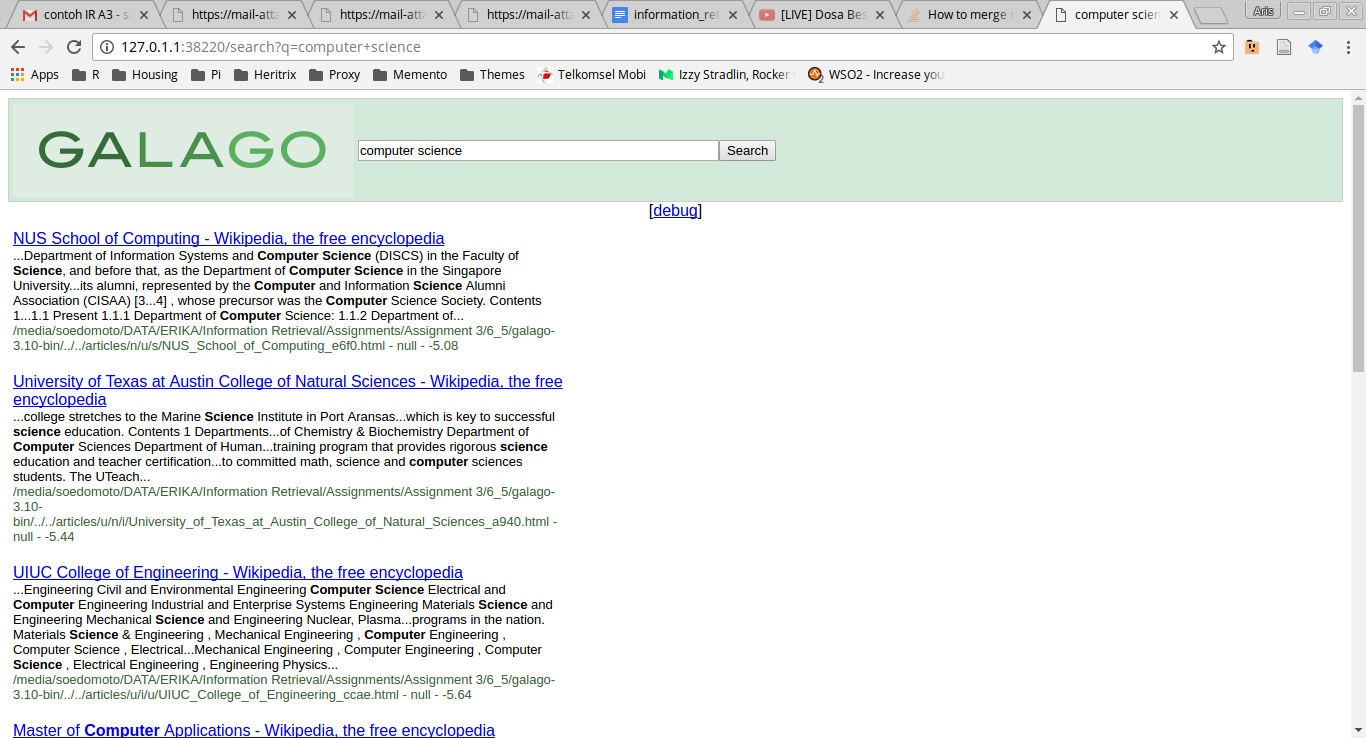
\includegraphics[width=\textwidth, height=\textheight, keepaspectratio]{computer_science}}
	\centering
	\caption{Snippet generated by Galago for query terms `computer science'}
	\label{fig:computer_science}
\end{figure}

Based on my analysis, I think Galago's snippet algorithm will not work well for pages with little text content. It is because the algorithm works by matching the query terms with the page content. If there is only little content on the page, then the probability to generate a good snippet will also decrease. 
One thing that we can use to improve the algorithm is to adopt the algorithm explained by Turpin \cite{Turpin:2007:FGR:1277741.1277766}. Turpin's algorithm does not only depends on the `matched terms'. It also uses the combination of several weights to improve the rank of the sentences such as the longest contiguous run of query terms and the position of the sentences. Figure \ref{fig:sentence_rank} illustrates the algorithm used by Turpin \cite{Turpin:2007:FGR:1277741.1277766} to generate snippets. 

\begin{figure}[H]
	\fbox{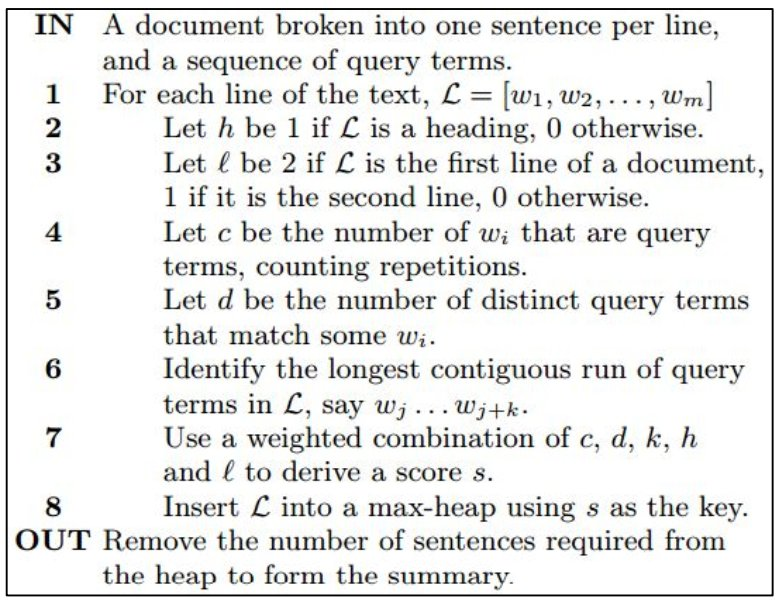
\includegraphics[scale=0.4]{sentence_rank}}
	\centering
	\caption{Turpin's algorithm for ranking the sentences. Adapted from \cite{Turpin:2007:FGR:1277741.1277766}}
	\label{fig:sentence_rank}
\end{figure}

\noindent\makebox[\linewidth]{\rule{\textwidth}{0.4pt}}

\section*{Question MLN1}
\begin{spverbatim}
MLN1: using the small wikipedia example, choose 10 words and create stem classes as per the algorithm on pp. 191-192.
\end{spverbatim}

\subsection*{Answer}

The steps to solve this problem is similar to what I have done in question 6.1. There are some differences:
\begin{enumerate}
\item There are 4 metrics that are use to measure the association between the terms, which are Dice's Coefficient, EMIM, MIM, and Chi-square. 
\item Window size = 100 words
\item Ten chosen words, which are \textit{daughter, army, provide, type, feature, free, standard, street, fin, and unit}. 
\end{enumerate}


Listing \ref{lst:mln1} shows the python code for this problem. 
\begin{lstlisting}[language=python, caption={Python code for MLN1}, label={lst:mln1}]

#!/usr/bin/python
import io
import math
import os
from krovetzstemmer import Stemmer as KrovetzStemmer

import html2text
import matplotlib.pyplot as plt
import networkx as nx
import nltk


# Create graph function
def create_graph(stem_data, metric_name):
    stemmed_word_data = {}
    for stemmed_word, word_a, word_b, coef in stem_data:
        stemmed_word_data.setdefault(stemmed_word, [])
        stemmed_word_data[stemmed_word].append((word_a, word_b, coef))

    stemmed_word_clusters = {}
    for stemmed_word, data in stemmed_word_data.items():
        G = nx.MultiGraph()

        labels = {}
        for word_a, word_b, coef in data:
            G.add_edge(word_a, word_b, weight=coef, label=coef)
            labels[(word_a, word_b)] = coef

        # export connected components into list
        stemmed_word_clusters[stemmed_word] = list(nx.connected_components(G))

        nx.draw(G, with_labels=True)
        nx.draw_networkx_edge_labels(G, pos=nx.spring_layout(G), edge_labels=labels)

        filename = '{}_graph_{}.png'.format(metric_name, stemmed_word)
        print('Saving graph {}'.format(filename))
        plt.savefig(filename, format='PNG')
        plt.clf()

    return stemmed_word_clusters


# Print stem cluster function
def print_stem_cluster(stemmed_word_clusters, metric_name):
    print('\n')
    print('Clusters using metric {}'.format(metric_name))
    print('==================================')

    for stemmed_word, connected_nodes in stemmed_word_clusters.items():
        for connected_node in connected_nodes:
            print(u'{}\t: {}'.format(stemmed_word, ', '.join(connected_node)))


# List all files ===========================================================================================
html_files = []
for root, dirs, files in os.walk(os.path.abspath('/media/erikaris/DATA/ODU/Semester 3/intro_to_info_retrieval/assignments/a2/code_report/articles/z')):
    for file in files:
        if file.endswith('.html'):
            filepath = os.path.join(root, file)
            html_files.append(filepath)


file_words_index = {}
all_words = set()
window_text_number = 100

# Index all words and files ================================================================================
for idx, file in enumerate(html_files):
    print('{} of {}. Processing file {}'.format(idx+1, len(html_files), file))
    print('=' * 30)

    # get text only from each file -> remove all tags
    h = html2text.HTML2Text()
    h.ignore_links = True
    text = h.handle(u' '.join([line.strip() for line in io.open(file, "r", encoding="utf-8").readlines()]))

    # get all words from text by splitting by whitespace
    words = [word.lower() for word in text.split() if word.isalpha()]

    # make text window containing 50 - 100 words
    for w in range(1, int(len(words)/window_text_number)):
        start = (w-1)*window_text_number
        end = w*window_text_number
        if end > len(words): end = len(words)

        window_words = words[start:end]

        all_words |= set(window_words)
        file_words_index[os.path.basename(file) + '_part_' + str(w)] = window_words


# # Remove stopword to purify result ========================================================================
# nltk.download('stopwords')
# all_words = [word for word in all_words if word not in stopwords.words('english')]
#
#
# # Select random 10 words ==================================================================================
# all_words = random.sample(all_words, 10)


# Invert words and files index ============================================================================
word_files_index = {}
for idx, word in enumerate(all_words):
    print('{} of {}. Processing word {}'.format(idx + 1, len(all_words), word.encode('utf-8')))
    print('=' * 30)

    files = []
    for file, words in file_words_index.items():
        if word in words:
            files.append(file)
    word_files_index[word] = sorted(set(files))


# Stem words ==============================================================================================
krovetz = KrovetzStemmer()
stem_word_index = {}
for word, files in word_files_index.items():
    # Stem word using krovetz
    stemmed_word = krovetz.stem(word)

    # Group by stemmed word
    stem_word_index.setdefault(stemmed_word, [])
    stem_word_index[stemmed_word].append(word)


# Calculate coefficient ==================================================================================
coef_threshold = 0.0

dice_stemmed_word_data = []
mim_stemmed_word_data = []
emim_stemmed_word_data = []
chi_sqr_stemmed_word_data = []

counter = 0
for stemmed_word, words in stem_word_index.items():
    # create bigrams from words
    bigrams = list(nltk.bigrams(words))
    for word_a, word_b in bigrams:
        # Lookup filename in word_files_index
        files_a = word_files_index[word_a]
        files_b = word_files_index[word_b]
        files_a_sliced_b = list(set(files_b) & set(files_a))

        # Using dice coef
        dice_coef = float(len(files_a_sliced_b)) / (len(files_a) + len(files_b))
        if (dice_coef > coef_threshold):
            dice_stemmed_word_data.append((stemmed_word, word_a, word_b, dice_coef))

        # Using MIM coef
        mim_coef = float(len(files_a_sliced_b)) / (len(files_a) * len(files_b))
        if (mim_coef > coef_threshold):
            mim_stemmed_word_data.append((stemmed_word, word_a, word_b, mim_coef))

        # Using EMIM coef
        if len(files_a_sliced_b) > 0:
            emim_coef = len(files_a_sliced_b) * \
                        math.log(len(file_words_index) * len(files_a_sliced_b) / float(len(files_a) * len(files_b)))
        else:
            emim_coef = 0.0

        if (emim_coef > coef_threshold):
            emim_stemmed_word_data.append((stemmed_word, word_a, word_b, emim_coef))

        # Chi-square
        chi_sqr_coef = math.pow((len(files_a_sliced_b) - (float(len(files_a) * len(files_b)) / len(file_words_index))), 2) / \
                       float(len(files_a) * len(files_b))
        if (chi_sqr_coef > coef_threshold):
            chi_sqr_stemmed_word_data.append((stemmed_word, word_a, word_b, chi_sqr_coef))

    if len(bigrams) > 0: counter+=1
    if counter >= 10: break



# Create graph
dice_stemmed_word_clusters = create_graph(dice_stemmed_word_data, 'dice')
mim_stemmed_word_clusters = create_graph(mim_stemmed_word_data, 'mim')
emim_stemmed_word_clusters = create_graph(emim_stemmed_word_data, 'emim')
chi_sqr_stemmed_word_clusters = create_graph(chi_sqr_stemmed_word_data, 'chi_sqr')

# Print clusters
print_stem_cluster(dice_stemmed_word_clusters, 'dice')
print_stem_cluster(mim_stemmed_word_clusters, 'mim')
print_stem_cluster(emim_stemmed_word_clusters, 'emim')
print_stem_cluster(chi_sqr_stemmed_word_clusters, 'chi_sqr')

\end{lstlisting}

I create the cluster using the graphs and extract the connected components from the graph. Figure \ref{fig:emim_graph_feature} shows the example of the graph for the word `feature'. 

\begin{figure}[H]
	\fbox{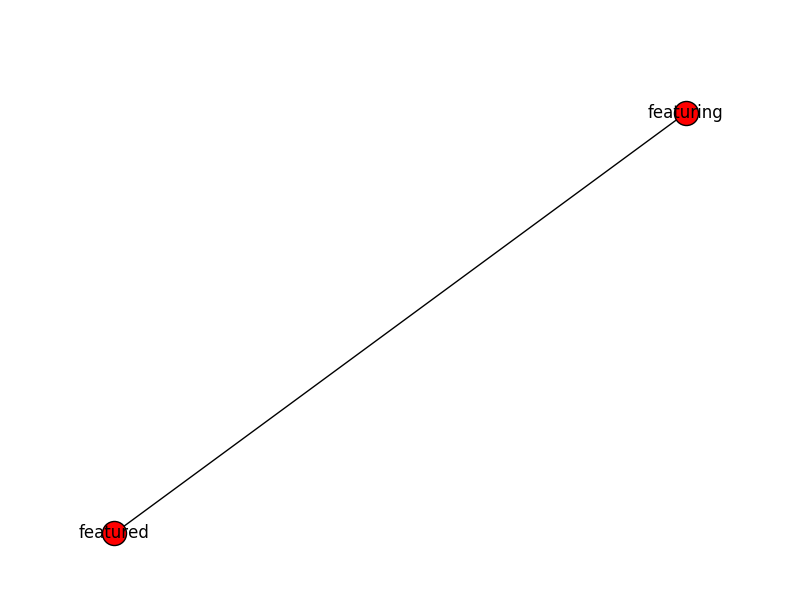
\includegraphics[scale=0.6]{emim_graph_feature}}
	\centering
	\caption{Connected component for the word `feature'}
	\label{fig:emim_graph_feature}
\end{figure}

From the output that I got, I see that difference association measurement return different clustering result. I also noticed that several terms do not have any other components connected to it. Figure \ref{fig:mln1_result} shows the cluster resulted from using Dice's Coefficient, MIM, EMIM, and Chi-square as the association measures. 

\begin{figure}[H]
	\fbox{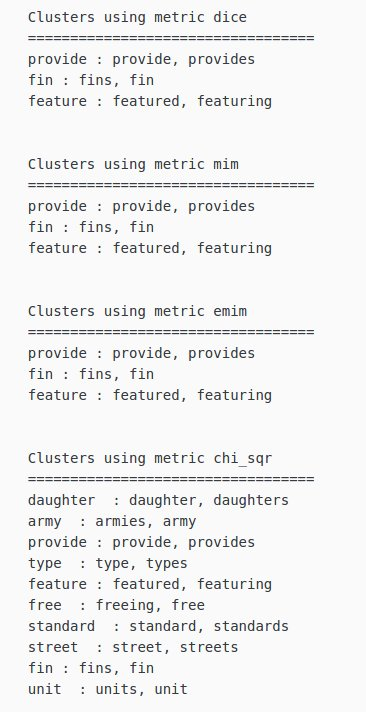
\includegraphics[scale=0.7]{mln1_result}}
	\centering
	\caption{The clustering result using Dice's Coefficient, MIM, EMIM, and Chi-square}
	\label{fig:mln1_result}
\end{figure}
    
\noindent\makebox[\linewidth]{\rule{\textwidth}{0.4pt}}


\section*{Question MLN2}
\begin{spverbatim}
MLN2: using the small wikipedia example, choose 10 words and compute MIM, EMIM, chi square, dice association measures for full document & 5 word windows (cf. pp. 203-205)
\end{spverbatim}

\subsection*{Answer}
e

\medskip

\bibliographystyle{unsrt}%Used BibTeX style is unsrt
\bibliography{biblio}

\end{document}
